\subsection{Kalibrierung der großen Scheibe}
Mit der großen Scheibe funktioniert die für die Winkelrichtgröße $D$ genauso wie für die kleine Scheibe. Aus diesem Grund werden hier nur die Werte (inkl. Fehler) angegeben. Es ergibt sich folgender Wert (Daten, siehe Abb. \ref{fig:kal2})
\begin{align*}
D = \unit[(2.17 \pm 0.04)]{N m}
\end{align*}
Die großen Fehlerwerte ergeben sich dadurch, dass die rücktreibende Kraft von der Richtung, in die die Scheibe ausgelenkt wird abhängt (materialbedingt).
\begin{figure}
\begin{center}
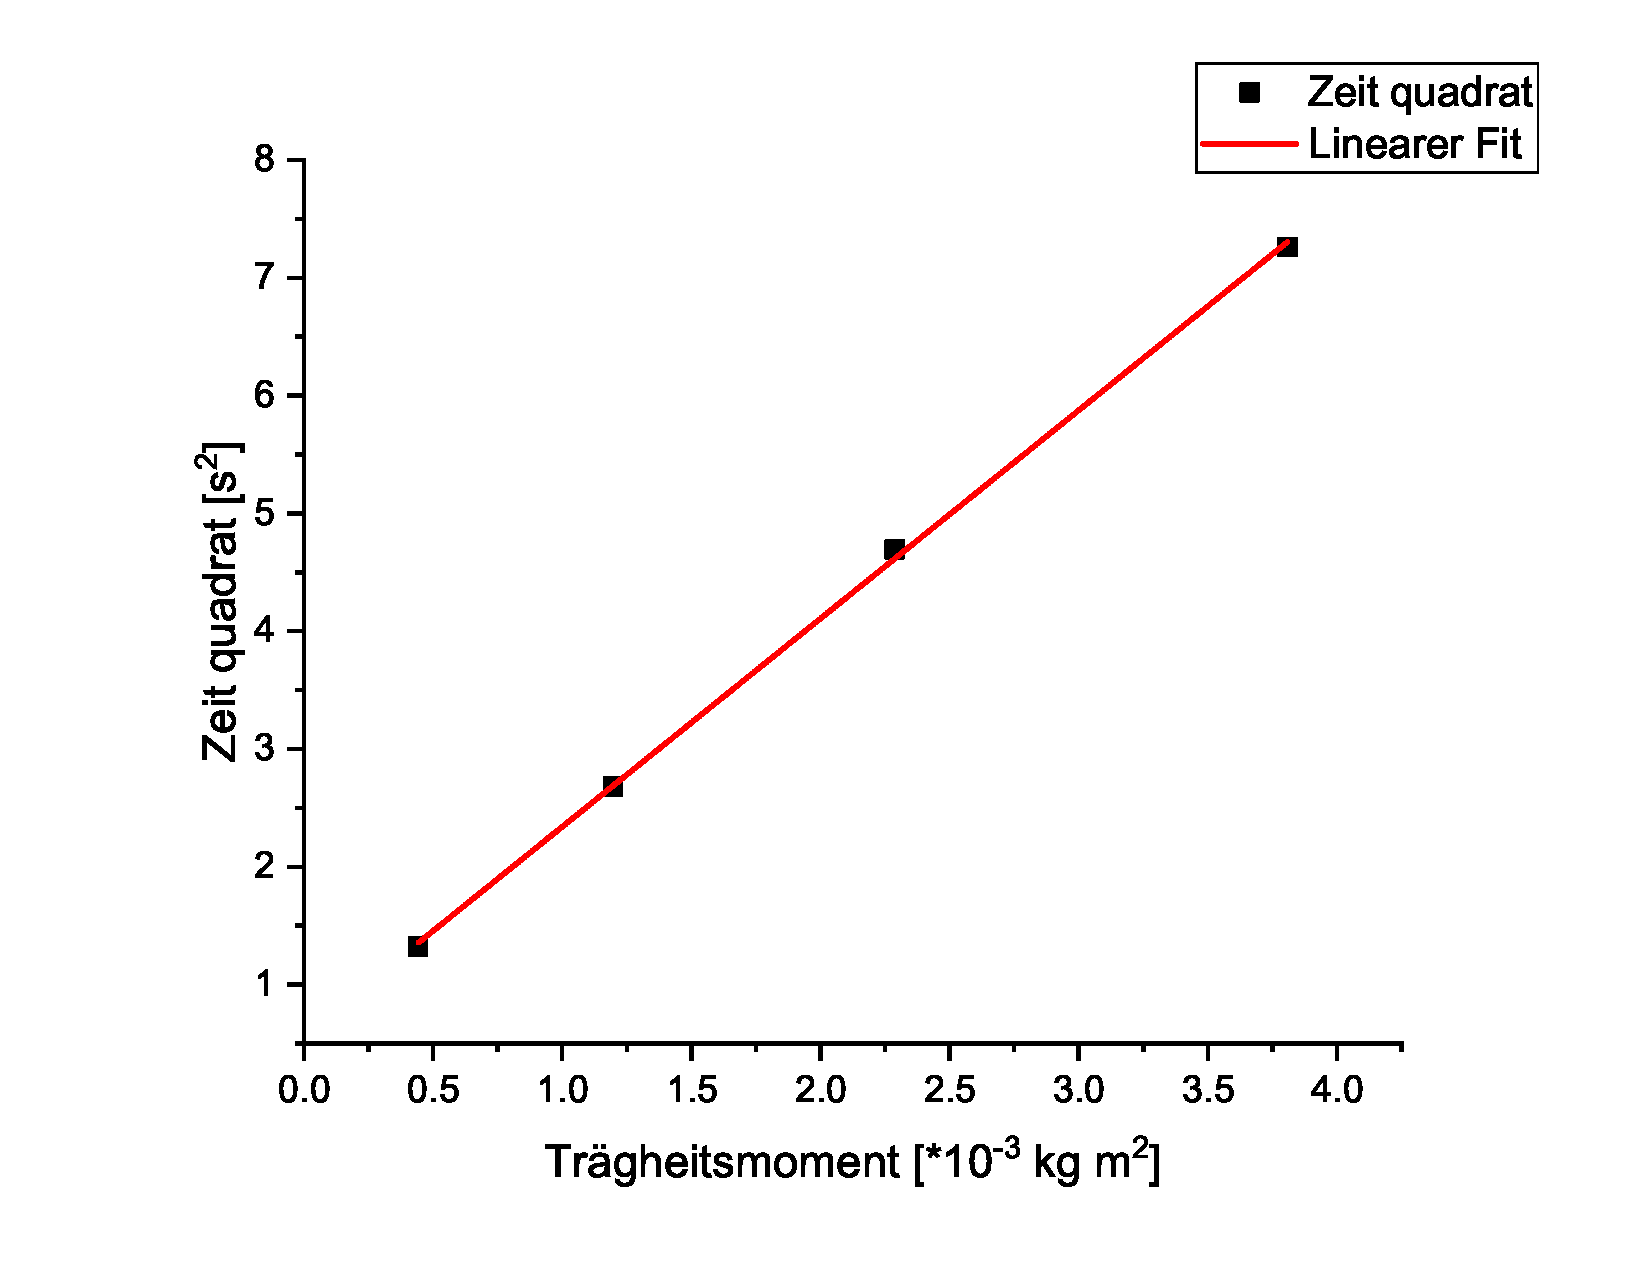
\includegraphics[width=0.7\textwidth]{Bilder/kal2.eps}
\caption{Kalibrierung der großen Scheibe}
\label{fig:kal2}
\end{center}
\end{figure}
Zudem ist das Material sowie die Abmessungen der Scheibe bekannt, also kann der Trägheitmoment berechnet werden:
\begin{equation}
J_0 = \frac{1}{2} m \cdot r^2 = \frac{1}{2} d\cdot r^2 \cdot \rho \pi r^2 = \unit[0.67]{kg m^2}
\end{equation}
Also ergibt sich für die Winkelrichtgröße $D = \unit{(2.27 \pm 0.3)]{N m}$.\\
Dieser relativ große Fehler ergibt sich durch die Ungenauigkeit im Radius, der mit der vierten Potenz in die Rechnung eingeht.






